\documentclass[10pt,ignorenonframetext,]{beamer}
\setbeamertemplate{caption}[numbered]
\setbeamertemplate{caption label separator}{: }
\setbeamercolor{caption name}{fg=normal text.fg}
\beamertemplatenavigationsymbolsempty
\usepackage{lmodern}
\usepackage{amssymb,amsmath}
\usepackage{ifxetex,ifluatex}
\usepackage{fixltx2e} % provides \textsubscript
%\usepackage[dvipdfmx]{graphicx}
\ifnum 0\ifxetex 1\fi\ifluatex 1\fi=0 % if pdftex
\usepackage[T1]{fontenc}
\usepackage[utf8]{inputenc}
\usepackage{epsfig}
\usepackage{mdframed}
\else % if luatex or xelatex
\ifxetex
\usepackage{mathspec}
\else
\usepackage{fontspec}
\fi
\defaultfontfeatures{Ligatures=TeX,Scale=MatchLowercase}
\fi
\usetheme{metropolis}
\usefonttheme{metropolis}
\usecolortheme{seahorse}
% use upquote if available, for straight quotes in verbatim environments
\IfFileExists{upquote.sty}{\usepackage{upquote}}{}
% use microtype if available
\IfFileExists{microtype.sty}{%
\usepackage{microtype}
\UseMicrotypeSet[protrusion]{basicmath} % disable protrusion for tt fonts
}{}
\newif\ifbibliography

% Prevent slide breaks in the middle of a paragraph:
\widowpenalties 1 10000
\raggedbottom

\AtBeginPart{
\let\insertpartnumber\relax
\let\partname\relax
\frame{\partpage}
}
\AtBeginSection{
\ifbibliography
\else
\let\insertsectionnumber\relax
\let\sectionname\relax
\frame{\sectionpage}
\fi
}
\AtBeginSubsection{
\let\insertsubsectionnumber\relax
\let\subsectionname\relax
\frame{\subsectionpage}
}

\setlength{\parindent}{0pt}
\setlength{\parskip}{6pt plus 2pt minus 1pt}
\setlength{\emergencystretch}{3em}  % prevent overfull lines
\providecommand{\tightlist}{%
\setlength{\itemsep}{0pt}\setlength{\parskip}{0pt}}
\setcounter{secnumdepth}{0}
\titlegraphic{\hfill
  
\includegraphics[height=1.5cm]{pictures/pobrane.png}
  
\includegraphics[height=1.5cm]{pictures/logoUG.jpg}
}
\usepackage{amsfonts} \usepackage{amssymb}
\usepackage{amsthm} \usepackage[MeX]{polski} \usepackage{graphicx}
\usepackage[skip=10pt]{caption} \usepackage{subcaption}
\usepackage{tikz} 
\usetikzlibrary{positioning}
\usetikzlibrary{arrows}
\usetikzlibrary{shapes.misc}
\usetikzlibrary{graphs}
\tikzset{main node/.style={circle,fill=blue!20,draw,minimum size=0.43m,inner sep=0pt},}
\tikzset{black node/.style={circle,fill=black,draw,minimum size=0.3cm,inner sep=0pt},}
\tikzset{white node/.style={circle,fill=white,draw,minimum size=0.3cm,inner sep=0pt},}
\tikzset{invisible node/.style={circle,fill=white,draw,opacity=0.01,minimum size=0.2cm,inner sep=0pt},}
\tikzset{cross/.style={cross out, draw=black, minimum size=2*(#1-\pgflinewidth), inner sep=0pt, outer sep=0pt, thick=2pt},cross/.default={0.2cm}}
\newtheorem{conj}{Conjecture} \newtheorem{obs}{Observation}
\newtheorem{corr}{Corollary} \newtheorem{exam}{Example}
\newtheorem{counterexam}{Counterexample}
\newtheorem{lem}{Lemma} \newtheorem{property}{Property}
\newtheorem{notation}{Notation} \newtheorem{probl}{Problem}
\newtheorem{operation}{Operation}


\usepackage{listings,lstautogobble}
\lstset{
	language=C,
	basicstyle=\small\sffamily,
	frame=tb,
	columns=fullflexible,
	showstringspaces=false,
	autogobble=true
}
\frenchspacing

\def\cer{{\rm cer}}

\title{Python: definicja świata i jego interakcji}
\subtitle{Podręcznik HOW-TO, czyli wprowadzenie co i jak}
\author{Opracowanie: Mateusz Miotk}
\date{01 Grudzień 2018}

\begin{document}
\frame{\titlepage}

\begin{frame}
Niniejszy podręcznik stanowi opracowanie niezbędne do przeprowadzania zajęć laboratoryjnych z tematyki \textbf{Python: definicja świata i jego interakcji}.
\end{frame}

\begin{frame}
Aby przystąpić do wykonywania ćwiczeń laboratoryjnych potrzebne są następujące rzeczy: 
\begin{itemize}
	\item Komputer stacjonarny (tutaj z systemem Linux)
	\item Terminal tekstowy 
	\item Język programowania Python + dowolne środowisko programistyczne obsługujące ten język
	\item Podstawy języka angielskiego
	\item Uczeń chętny do pracy :-) 
\end{itemize}
\begin{figure}[!h]
	\centering
	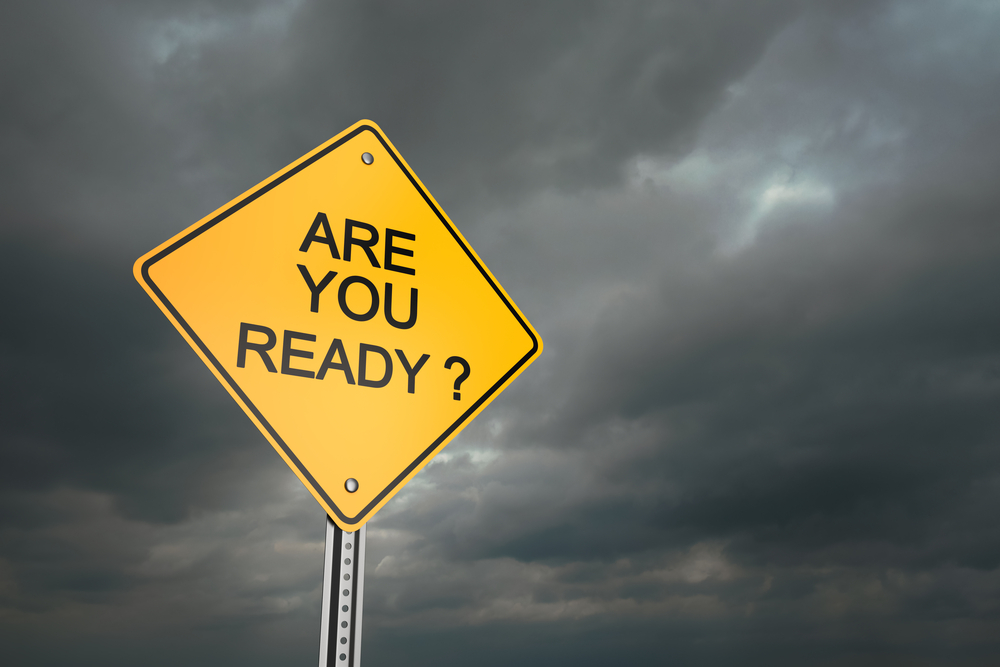
\includegraphics[scale=0.75]{pictures/ready.jpeg}
\end{figure}
\end{frame}

\begin{frame}{Pierwsze kroki - logowanie do systemu}
  Aby przystąpić do realizacji zadań należy wybrać system Linux (z poziomu menu), a następnie zalogować poprzez login i hasło (które zostało przekazane przez prowadzącego). 
  
  Logowanie odbywa się poprzez wybór \textbf{Inny użytkowinik} i wtedy wpisujemy login i hasło.
\end{frame}

\begin{frame}{Pierwsze kroki - zapoznanie się z systemem Linux}
  W wyniku poprawnego zalogowania otrzymamy pulpit w systemie Linux.
  
  Jednym z podstawowych narzędzi, które używa się w systemie Linux jest \textbf{emulator terminala tekstowego} i wygląda on przykładowo następująco: 
  
  \begin{figure}[!h]
  	\centering
  	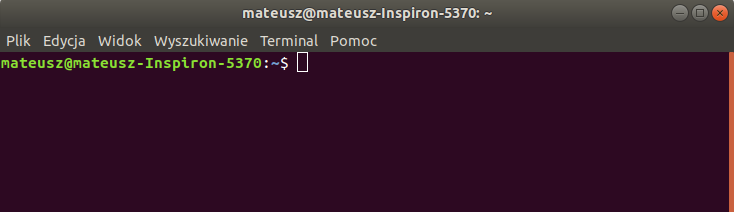
\includegraphics[scale=0.45]{pictures/terminal.png}
  \end{figure}
  Powyższe narzędzie znajdziesz klikając \textbf{menu -> akcesoria -> emulator terminala}.
\end{frame}

\begin{frame}{Pierwsze kroki - podstawowe komendy systemu Linux}
  Tutaj wymienione zostały podstawowe komendy, które stosuje się w terminalu tekstowym systemu Linux:	
  \begin{itemize}
  	\item ls - wyświetlenie zawartości katalogu domowego
  	\item pwd - wyświetlenie ścieżki w obecnym miejscu
  	\item cd <nazwa folderu> - przejście do folderu o nazwie <nazwa folderu>
  	\item touch <nazwa pliku> - stworzenie pliku o nazwie <nazwa pliku>
  	\item mkdir <nazwa katalogu> - stworzenie katalogu o nazwie <nazwa katalogu>
  	\item rm <nazwa pliku> - usuwanie pliku o nazwie nazwa pliku
  	\item cp <plik> <plik2> - kopiowanie pliku o nazwie plik do pliku o nazwie plik2
  	\item nano <nazwa pliku> - otwarcie programu nano (edytora tekstowego coś jak notatnik) dla pliku o nazwie nazwa pliku
  \end{itemize}
\end{frame}

\begin{frame}{Pierwsze kroki - język programowania Python}
  Aby uruchomić konsolę Pythona należy użyć następującego polecenia: \textbf{python3}. 
  
  W wyniku otrzymamy następujący widok terminala (może różnić się kolorami): 
  \begin{figure}[!h]
  	\centering
  	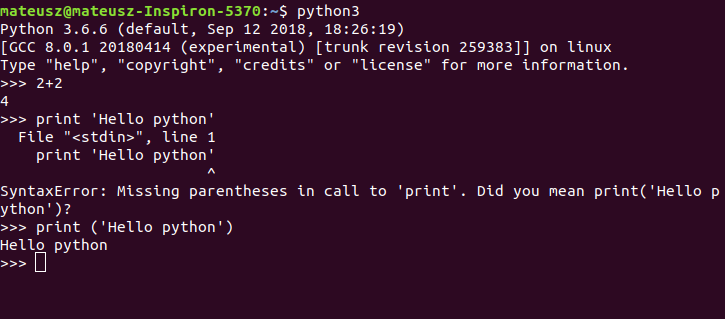
\includegraphics[scale=0.45]{pictures/python.png}
  \end{figure}
\end{frame}

\begin{frame}{Pierwsze kroki - język programowania Python}
  Program w języku python można też uruchamiać przy pomocy polecenia \textbf{python3} nazwapliku.py
  
  Rozszerzeniem dla programów napisanych w języku \textbf{Python} jest \textbf{.py}.
  
  Rozważmy plik \textbf{hello.py}, w którym mamy następujący kod programu napisany w języku Python: 
  
    \begin{figure}[!h]
  	\centering
  	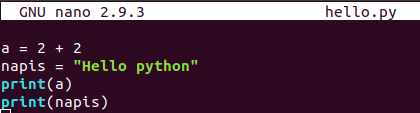
\includegraphics[scale=0.35]{pictures/helloPy.png}
  \end{figure}
  Wynik napisanego programu wygląda następująco: 
    \begin{figure}[!h]
  	\centering
  	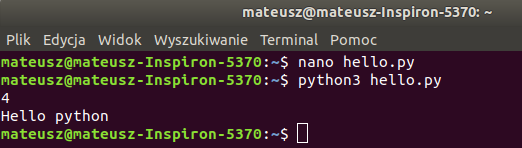
\includegraphics[scale=0.35]{pictures/outputPython.png}
  \end{figure}
\end{frame}

\begin{frame}{Pierwsze kroki - środowisko programistyczne Visual Studio Code}
  Aby ułatwić sobie życie w programowaniu można użyć środowiska programistycznego. Istnieje szeroki wybór między środowiskami programistycznymi. 
  Tutaj podany jest przykład użycia środowiska Visual Studio Code (dostępny w menu -> programowanie -> Visual Studio Code): 
      \begin{figure}[!h]
  	\centering
  	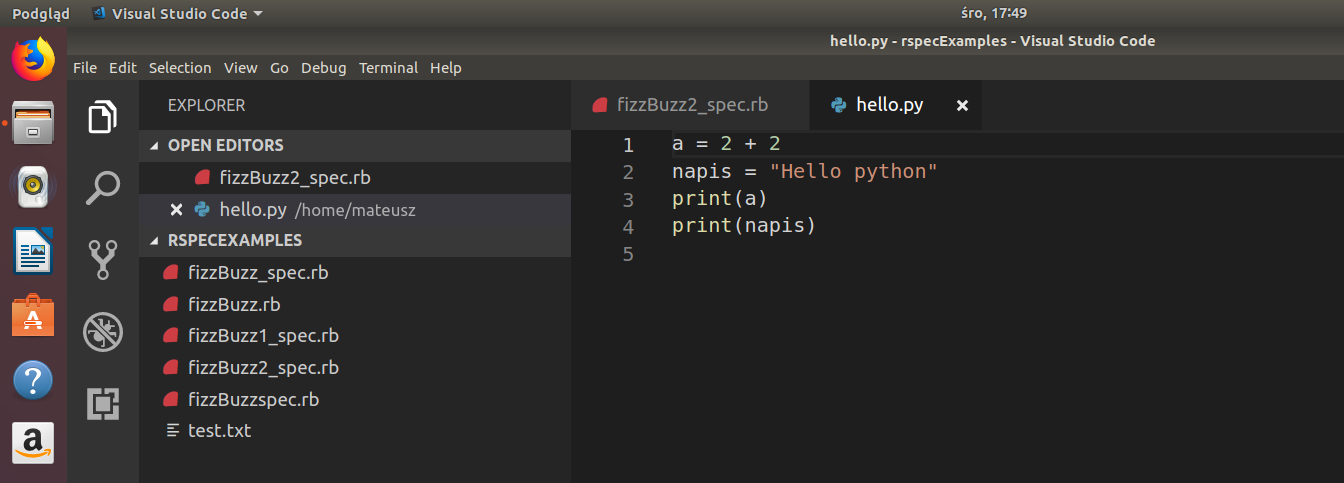
\includegraphics[scale=0.25]{pictures/visual.png}
  \end{figure}
\end{frame}

\begin{frame}{Pierwsze kroki - pobieranie zadań przy pomocy narzędzia wget}
  Aby pobrać zadania laboratoryjne należy wykonać następujące rzeczy: 
  \begin{itemize}
  	\item Otworzyć terminal tekstowy
  	\item Wpisać następującą komendę: wget https://inf.ug.edu.pl/~mmiotk/PythonWorld-master.zip
  	\item Wpisać komendę: unzip -qq PythonWorld-master.zip
  	\item Pojawi się katalog PythonWorld-master
  \end{itemize}
      \begin{figure}[!h]
	\centering
	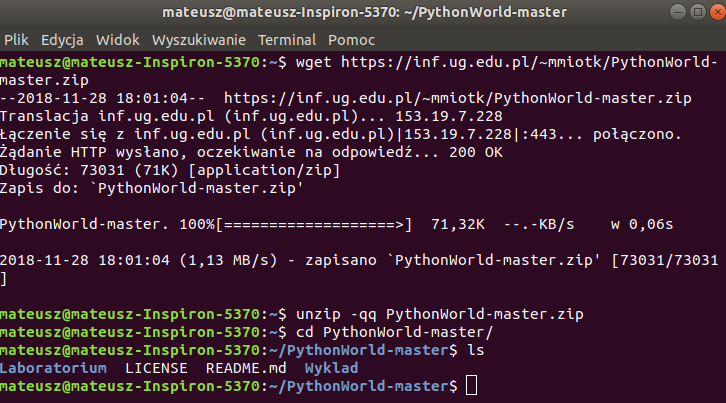
\includegraphics[scale=0.3]{pictures/pobieranie.png}
\end{figure}
\end{frame}

\begin{frame}{Pierwsze kroki - uruchamianie świata}
  Aby uruchomić program/świat należy użyć komendy python3 Main.py (patrz screen poniżej): 
        \begin{figure}[!h]
  	\centering
  	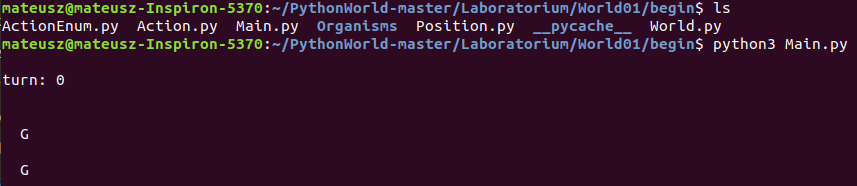
\includegraphics[scale=0.35]{pictures/runworld.png}
  \end{figure}
\begin{center}
	\textbf{POWODZENIA W ŚWIECIE PROGRAMOWANIA!!!}
\end{center}

\end{frame}

\begin{frame}{Thank you!}
\begin{figure}[!h]
	\begin{center}
		
\includegraphics[scale=0.4]{pictures/thank.jpg}
	\end{center}
\end{figure}
\end{frame}

\end{document}